\section{Methods}

\subsection{Glycan Hypothesis Generation}
    In eukaryotes, \nglycans start with a common, conserved core of \textbf{HexNAc2 Hex3},
    building up to \textbf{HexNAc2 Hex9} (\cite{Stanley2009}). This structure is refined by
    sequentially removing monosaccharides and replacing them with more complex structures
    through a series of glycosidase and glycosyltransferase reactions, the enumeration of
    which as shown in \cite{Akune2016} yields over a million of possible \nglycan topologies
    and epitopes. These topologies define the geometry of the glycan, affecting the glycan's
    binding affinities and how the glycan may influence protein folding and accessibility,
    the glycan's functional aspects. The medium through which we observe \nglycan does not
    capture the full tree or graph structure of an \nglycan, so we reduce the topology to
    a count of each type of residue.

    Starting with the core motif, we generate all combinations of monosaccharides ranging
    between the limits in Table \ref{tbl:glycan_composition_rules}. We created a copy of
    this database for native, reduced and permethylated, and deuteroreduced and permethylated.
    Let $n = 1240$ be the number of glycan compositions $\mathbf{g}$ in the database.

    \renewcommand{\arraystretch}{1.5}
    \begin{table}
        \centering
        \caption{Glycan Composition Rule Table}\label{tbl:glycan_composition_rules}
        \begin{tabular}{c | c | c | c}
            Monosaccharide & Lower Limit & Upper Limit & Constraints\\
            \hline
            \monosaccharide{HexNAc} & 2 & 9 &\\
            \monosaccharide{Hex} & 3 & 10 & \\
            \monosaccharide{Fuc} & 0 & 4 & $\monosaccharide{HexNAc} > \monosaccharide{Fuc}$\\
            \monosaccharide{NeuAc} & 0 & 5 & $(\monosaccharide{HexNAc} - 1) > \monosaccharide{NeuAc}$\\
        \end{tabular}
    \end{table}
    \renewcommand{\arraystretch}{1.0}

\subsection{LC-MS Data Preprocessing}
    We used samples from several sources including both QTOF and FTMS instruments as shown
    in Table \ref{tbl:sample_overview}. For details on sample preparation and data acquisition,
    please see their source citation. All data were converted into mzML format (\cite{Martens2011})
    prior to analysis with Proteowizard (\cite{Kessner2008}) without any data transforming filters.
    We applied a background reduction method based upon (\cite{Kaur2006}), using a window length
    of 2 m/z. Next, we picked peaks using a simple gaussian model. Scans were then subjected
    to iterative charge state deconvolution and deisotoping using an averagine (\cite{Senko1995})
    formula appropriate to the molecule under study. For native glycans, the formula was
    \textbf{H 1.690 C 1.0 O 0.738 N 0.071}, for permethylated glycans, the formula was
    \textbf{H 1.819 C 1.0 O 0.431 N 0.042}. We used an iterative approach which combines
    aspects of the dependence graph method (\cite{Liu2010}) and with subtraction. All samples
    were processed using a minimum isotopic fit score of 35 with an isotopic strictness penalty
    of 2.

    \renewcommand{\arraystretch}{1.5}
    \begin{table}
        \caption{Samples Used}\label{tbl:sample_overview}
        \centering
        \begin{tabular}{p{4cm} | c | p{3cm} | p{3cm} | c}
            Sample Name & Instrument & Derivatization & Adduction & Source\\
            \hline
            20150930-06-AGP & QTOF & Native & Formate (1) & \cite{Khatri2016a}\\
            20141031-07-Phil-82 & QTOF & Native & Formate(3) & \cite{Khatri2016a}\\
            20141101-04-Phil-BS & QTOF & Native & Formate(3) & \cite{Khatri2016a}\\
            20151002-02-IGG & QTOF & Native & Formate (2) & \cite{Khatri2016b}\\
            20141128-11-Phil-82 & QTOF & Deutero-reduced and Permethylated & Ammonium (3) & \cite{Khatri2016a}\\
            AGP-DR-Perm-glycans-1 & FTMS & Deutero-reduced and Permethylated & Ammonium (3) & \cite{Khatri2016a}\\
            AGP-permethylated-2ul-inj-55-SLens & FTMS & Reduced and Permethylated & Ammonium (3)
                                                      & \cite{Khatri2016a}\\
            Perm-BS-070111-04-Human-Serum & FTMS & Reduced and Permethylated & Ammonium (3) & \cite{Yu2013}\\
        \end{tabular}
    \end{table}
    \renewcommand{\arraystretch}{1.0}

\subsection{Chromatogram Aggregation}
    We clustered peaks whose neutral masses were within 15 parts-per-million error
    (PPM) of each other. When there were multiple candidate clusters for a single peak,
    we used the cluster with the lowest mass error. After all peaks were clustered,
    we sorted each cluster by time, creating a list of aggregated chromatograms. To account
    for small mass differences, we found all chromatograms 

\subsection{Glycan Composition Matching}
    For each chromatogram, we queried the target glycan database for compositions whose
    masses were within $\delta_{mass} = 10$ PPM mass error for QTOF data, $5$ PPM mass error
    for FTMS data. We merged all features matching the same composition. Then, for
    each adduct combination, we searched the target glycan database for compositions
    whose neutral mass were within $\delta_{mass}$ of the observed neutral mass - adduct
    combination mass, followed by another round of merging chromatogramss with the same
    assigned composition. We reduced the data by splitting each feature where the time
    between sequential observation was greater than $\delta_{rt} = 0.25$ minutes and
    removed features with fewer than $k = 5$ data points. We term the remaining assigned
    and unassigned chromatograms {\em candidate features}.

% This section runs quite long but is necessary to define the "Observed Score"
% which the network smoothing method is supposed to smooth over. I doubt I'll be
% able to include all of this section, the definition of the steps involved in
% defining the network, and the network smoothing itself.
\subsection{Feature Evaluation}
    For each candidate feature, we computed several statistics to estimate how distinguishable
    the observed signal was from random noise. We use the following quantities from each LC-MS
    feature:

    \renewcommand{\arraystretch}{1.5}
    \begin{table}
        \caption{Chromatogram Feature Definitions}\label{tbl:chromatogram_feature_definitions}
        \centering
        \begin{tabular}{l | p{9cm}}
            \hline
            $\mathcal{M}_i$ & The neutral mass of the $i$th chromatogram\\
            $\mathbfcal{I}_i$ & The total intensity array assigned to the $i$th chromatogram\\
            $\mathbfcal{I}_{i, j}$ & The sum of all peak intensities for peaks observed in
                                             the $j$th scan for the $i$th chromatogram\\
            $\mathcal{I}_{i, j, k}$ & The intensity assigned to the $k$th peak at the $j$th
                                      scan for the $i$th chromatogram\\
            $\mathbf{c}_i$ & The set of charge states observed for the $i$th chromatogram\\
            $\mathbfcal{I}_{i, c=j}$ & The total intensity assigned to the $i$th chromatogram
                                     with charge state $j$\\
            $\mathbf{t}_{i, j}$ & The time of the $j$th scan of the $i$th chromatogram\\
            $\textbf{env}_{i, j, k}$ & The normalized experimental isotopic envelope composing
                                     the $k$th peak of the $j$th scan of the $i$th chromatogram,
                                     whose members sum to $1$\\
            $\mathbf{a}_i$ & The set of adduction states observed for the $i$th chromatogram\\
            $\mathbfcal{I}_{i, a=j}$ & The total intensity assigned to the $i$th
                                                 chromatogram with adduct $j$\\
            ${\hat g}_i$ & The glycan composition assigned to the $i$th chromatogram, or \O
                           \ if there was no matched glycan composition
        \end{tabular}
    \end{table}
    \renewcommand{\arraystretch}{1.0}

    \subsubsection{Chromatographic Peak Shape}
        An LC-MS elution profile should be composed of one or more peak-like components, each
        following a bi-Gaussian peak shape model (\cite{Yu2010}) or in less ideal chromatographic
        circumstances, a skewed Gaussian peak shape model. We fit these models using non-linear
        least squares (NLS). As measures of goodness of fit are not generally available for NLS,
        we use the following criterion:
        \begin{align}
            {\hat y_i} &= NLS(\mathbfcal{I}_i, \mathbf{t}_i) \nonumber\\
            e_{i, NLS} &= \mathbfcal{I}_i - {\hat y_i} \nonumber\\
            {\bar y_i} &= \mathbf{t}_i
                \left(
                    \left(
                        \mathbf{t}_i^t\mathbf{t}_i
                    \right)^{-1}\mathbf{t}_i\mathbfcal{I}_i
                \right)\nonumber\\
            e_{i, null} &= \mathbfcal{I}_i - {\bar y_i} \nonumber\\
            \mathscr{L}_i &= 1 - \frac{\sum{e_{i, NLS}^2}}{\sum{e_{i, null}^2}}
        \end{align}
        \noindent where line score describes how much the peak shape fit improves on a straight
        line fit null model.

        % Likely to be moved to the supplement
        We apply two competitive peak fitting strategies to address distorted, overlapping, or
        multimodal elution profiles. The first works iteratively by finding a best-matching peak
        shape using non-linear least squares, subtracting the fitted signal and checks if there is
        another peak with at least half as tall as the removed peak, if so repeating the process until
        no peak can be found, saving each peak model so constructed. The second approach starts
        by locating local minima between putative peaks, and partitioning the chromatogram into
        sub-groups which would are fit independently. This method generates a candidate list of
        minima, and selects the case which has the greatest difference between the minimum and its
        pair of maxima to split the feature at. The strategy which produces the maximum $\mathscr{L}_i$
        is chosen.

    \subsubsection{Composition Dependent Charge State Distribution}
        % Does this principle need a citation?
        As the number of monosaccharides composing a glycan increases, the number of possible sites
        for charge localization increases. Under normal conditions, we would expect to observe the
        same molecule in multiple charge states (\cite{Maxwell2012}). Which charge states are
        expected would depend upon the size of the molecule and it's constituent units'
        electronegativity. In it's native state, \monosaccharide{NeuAc}'s acidic group causes
        glycans with one or more \monosaccharide{NeuAc} to have a propensity for higher negative
        charge states (\cite{Varki2009}). To capture this relationship, we modeled the probability of
        observing a glycan composition for sialylated and unsialylated compositions separately. For
        permethylated glycans, charge is carried by protons or metallic cation adducts like sodium,
        the relationship between acidic monosaccharides and charge state propensities is weaker.

        \begin{align}
            m_i &= (\floor*{(\mathcal{M}_i / w) / 10} + 1) * 10 \nonumber\\
            \mathcal{H}_{i,j} &= \frac{
                \mathbfcal{I}_{i, c=j}}{\mathbfcal{I}_i} \nonumber\\
            P(c, m) &= |m|\sum_{m_i \in m} \mathcal{H}_{i, j} \nonumber\\
            \mathscr{C}_i &= \sum_{c_{i, j} \in \mathbf{c}_i}{P(c_{i, j}, m_i)}
        \end{align}

        \noindent where $w$ is the width of the mass bin divided by 10 and $P(c, m)$ is defined as
        part of the model estimation procedure.

        \begin{figure}
            \centering
            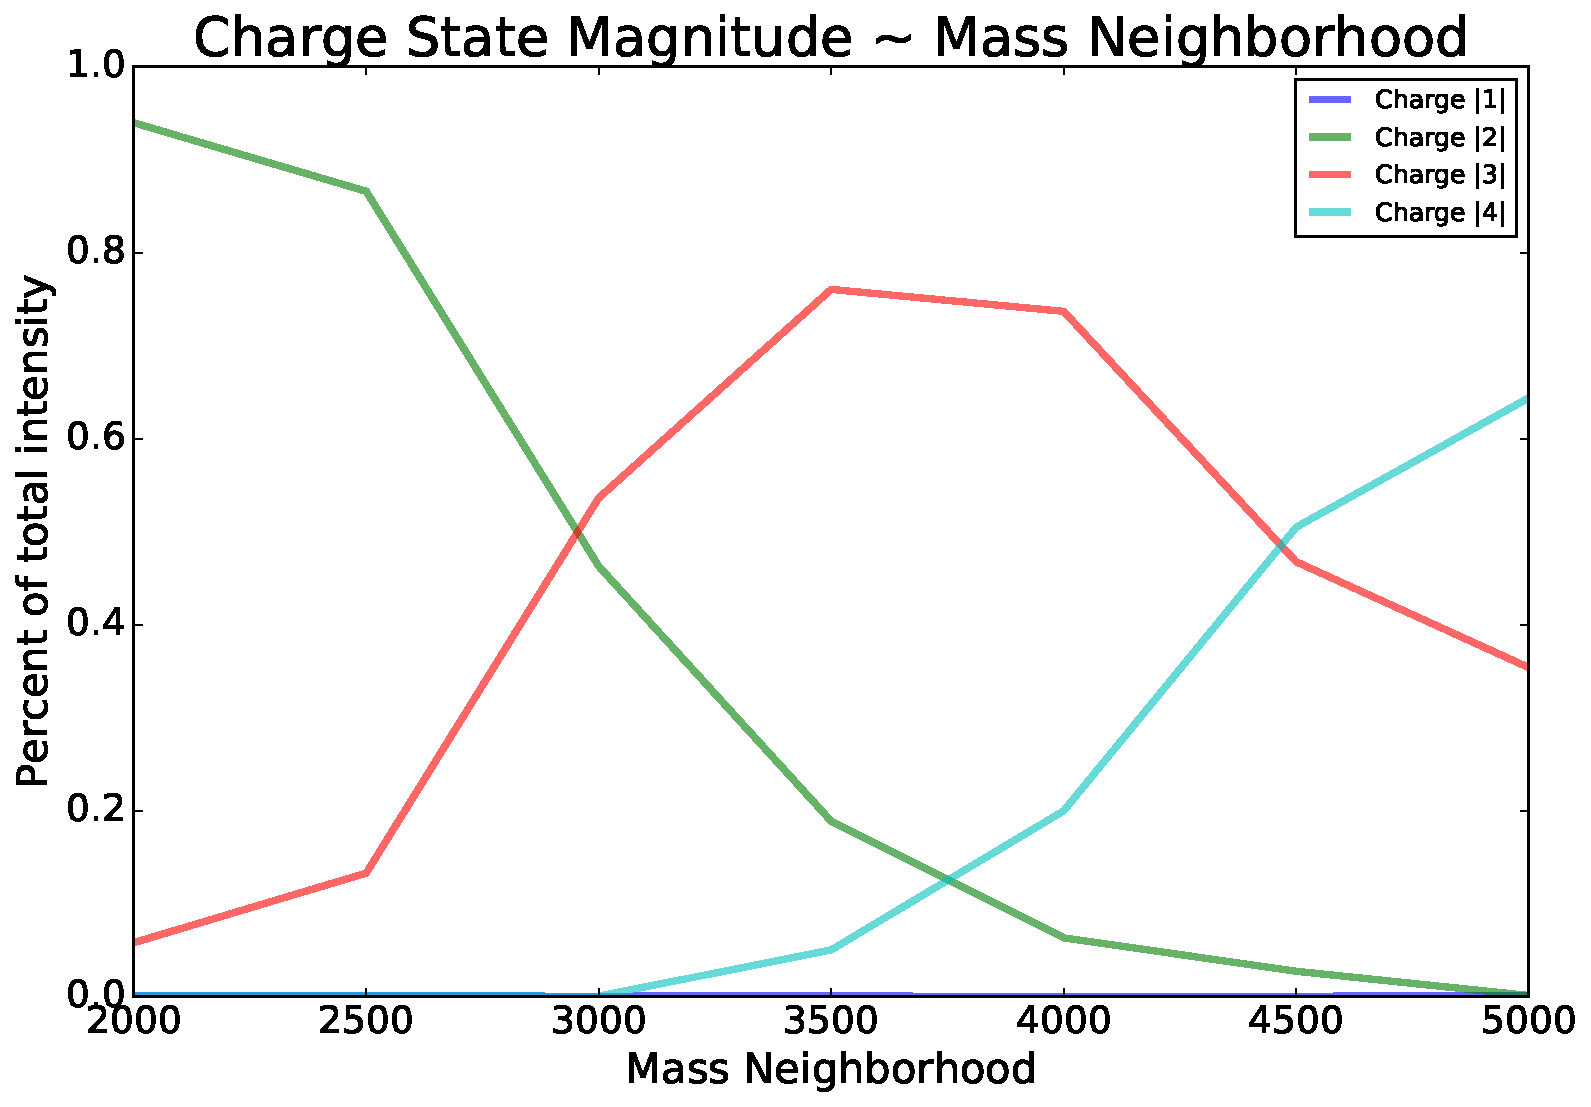
\includegraphics[width=0.75\linewidth]{figure/charge_trend_plot}
            \caption{The trend of charge state relative abundance for acidic glycans}
            \label{fig:charge_trend_plot}
        \end{figure}

    \subsubsection{Adduction Rate}
        For the samples \textit{AGP-permethylated-2ul-inj-55-SLens} and \textit{Perm-BS-070111-04-Human-Serum}
        we also include an Adduction Frequency model score $\mathscr{A}_i$, following the same
        pattern as the charge state distribution, with the same extension of justification
        from \cite{Maxwell2012}. We use one mass scaling model for all glycan compositions
        as ammmonium adduction is not expected to be composition dependent.

        \begin{align}
            \mathcal{H}_{i,j} &= \frac{
                \mathbfcal{I}_{i, a=j}}{\mathbfcal{I}_i} \nonumber\\
            P(a, m) &= |m|\sum_{m_i \in m} \mathcal{H}_{i, j} \nonumber\\
            \mathscr{A}_i &= \sum_{a_{i, j} \in \mathbf{a}_i}{P(a_{i, j}, m_i)}
        \end{align}

        We fit the adduction rate model on \textit{AGP-permethylated-2ul-inj-55-SLens} in order
        to make our comparison to third-party data less biased given limited sample data.

    \subsubsection{Isotopic Pattern Consistency}
        Our ahead-of-time deconvolution procedure uses an averagine isotopic model and does not
        capture the consistency of the isotopic pattern that was fit with the isotopic pattern
        of the glycan composition that matched that peak. The criterion
        \begin{align}
            \mathscr{I}_i &= 1 - 2\mathbfcal{I}_i^{-t}\mathbf{I}_i\sum_j^J{
                \sum_k^K{\mathcal{I}_{i, j, k}
                    \textbf{env}_{i, j, k}^t\left(
                        \ln{\textbf{env}}_{i, j, k} -
                        \ln{\textbf{tid}_{i}}
                    \right)
                }
            }
        \end{align}
        \noindent where \textbf{tid} is the theoretical isotopic pattern derived from either ${\hat g}_i$
        or an averagine interpolated for $\mathcal{M}_i$ if ${\hat g}_i =$ \O. This computes a
        per-peak intensity weighted mean G-test comparing the goodness of fit between the experimental
        envelope and the theoretical isotopic pattern.

    \subsubsection{Observation Spacing Score}
        The less time between observations of a glycan composition the less likely the chromatogram
        is to contain peaks missing or caused by isotopic pattern interference or missing information.
        \begin{align}
            \mathscr{T}_i &= 1 - 2\mathbfcal{I}_i^{-t}\mathbf{I}_i\sum_{j=1}^J\mathbfcal{I}_{i, j}(
                \mathbf{t}_{i, j} - \mathbf{t}_{i, j - 1})
        \end{align}

    \subsubsection{Summarization Score}
        Each scoring feature $\in \left[\mathscr{L}_i, \mathscr{C}_i, \mathscr{I}_i,
        \mathscr{T}_i\right]$ is penalized by $\epsilon = 1\mathrm{e}{-6}$ bounded in
        the range $[0, 1)$, with values below 0 set to $\epsilon$.

        \begin{align}
            s_i &= \sum_{f_{i,j} \in \text{features}_i}{\ln{
                \frac{f_{i, j}}{1 - f_{i, j}}
                }
            }
        \end{align}

        \noindent producing a value between $(-\infty, \infty)$. $s_i < 8$ reflects multiple
        poor feature scores and is unexpected to be real, while $s_i > 15$ is
        consistent with model expectations.

\subsection{Glycan Composition Network Smoothing}
    Evidence for individual glycan compostions can often be enough to claim that
    composition had been detected. Lower abundance may score poorly in one or
    more features, leading to the glycan composition being discarded. Other
    methods have demonstrated it is advantageous to use relationships between
    glycans based on biosynthetic or structural rules to adjust the score of a
    single glycan assignment (\cite{Goldberg2009, Kronewitter2014}). This idea
    has been explored more generically under the name "Manifold Regularization"
    (\cite{Belkin2006}) and specifically "Laplacian Regularization" when the
    Laplacian matrix of a graph is used to influence the parameter scaling. We
    apply this idea to weighted networks of related glycans with arbitrarily
    defined and overlapping sub-populations.

    \subsubsection{Glycan Composition Graph}
        For each database of theoretical glycan compositions we create, we
        define each composition to be a coordinate vector in a $\mathcal{Z}^{+4}$
        space, and represented by a node in an undirected glycan composition
        graph $\mathcal{G}$. Under this interpretation, we can compute the
        $L_1$-distance between two glycan compositions. For any two glycan
        compositions $g_u, g_v$, if $L_1(g_u, g_v) = 1$ we add an edge
        connecting $g_u$ and $g_v$ to $\mathcal{G}$ with weight $w = 1$.

    \subsubsection{Neighborhood Definition}
        Our definition of distance connects glycan compositions which differ
        by a single monosaccharide, but we can assert larger collections of
        glycan compositions are related. We define the following neighborhoods
        for {\em N}-glycans:

        \begin{table}
            \centering
            \begin{tabular}[h]{l | p{8cm}}
                Name & Bounds \\
                \hline
                High Mannose & $\monosaccharide{HexNAc} = 2 \land
                                \monosaccharide{Hex} \in [3, 10]
                                \land \monosaccharide{NeuAc} = 0$\\
                Hybrid & $\monosaccharide{HexNAc} \in [2, 4] \land
                          \monosaccharide{Hex} \in [2, 6]
                          \land \monosaccharide{NeuAc} \in [0, 2]$\\
                Bi-Antennary & $\monosaccharide{HexNAc} \in [3, 5]
                                \land \monosaccharide{Hex} \in [3, 6]
                                \land \monosaccharide{NeuAc} \in [1, 3]$\\
                Asialo-Bi-Antennary & $\monosaccharide{HexNAc} \in [3, 5]
                                \land \monosaccharide{Hex} \in [3, 6]
                                \land \monosaccharide{NeuAc} \in [0, 1]$\\
                Tri-Antennary & $
                    \monosaccharide{HexNAc} \in [4, 6]
                    \land \monosaccharide{Hex} \in [4, 7]
                    \land \monosaccharide{NeuAc} \in [1, 4]
                $\\
                Asialo-Tri-Antennary & $
                    \monosaccharide{HexNAc} \in [4, 6]
                    \land \monosaccharide{Hex} \in [4, 7]
                    \land \monosaccharide{NeuAc} \in [0, 0]
                $\\
                Tetra-Antennary & $
                    \monosaccharide{HexNAc} \in [5, 7]
                    \land \monosaccharide{Hex} \in [5, 8]
                    \land \monosaccharide{NeuAc} \in [1, 5]
                $\\
                Asialo-Tetra-Antennary & $
                    \monosaccharide{HexNAc} \in [5, 7]
                    \land \monosaccharide{Hex} \in [5, 8]
                    \land \monosaccharide{NeuAc} \in [0, 0]
                $\\
                Penta-Antennary & $
                    \monosaccharide{HexNAc} \in [6, 8]
                    \land \monosaccharide{Hex} \in [6, 9]
                    \land \monosaccharide{NeuAc} \in [1, 5]
                $\\
                Asialo-Penta-Antennary & $
                    \monosaccharide{HexNAc} \in [6, 8]
                    \land \monosaccharide{Hex} \in [6, 9]
                    \land \monosaccharide{NeuAc} \in [0, 0]
                $
            \end{tabular}
            \caption{N-Glycan Neighborhoods}
            \label{tbl:neighborhood_definitions}
        \end{table}

        Glycan compositions may belong to zero or more neighborhoods,
        as there are unusual glycan compositions which do not satisfy
        any neighborhood's rules, and several neighborhoods intentionally
        overlap to express broad relationships between groups. We define
        a matrix $\mathbf{A}$ as an $n \times k$ matrix where $A_{i, k}$
        to be the degree to which $g_i$ belongs $k$th neighborhood:

        \begin{align}
            A_{i, k} &= \frac{1}{|\text{neighborhood}_k|}\sum_{
                g^* \in \text{neighborhood}_k}{L_1(g_i, g^*)}
        \end{align}

        To reduce the impact of neighborhood size on the elements
        of $\mathbf{A}$, the columns of $\mathbf{A}$ are first
        normalized to sum to 1, and then the rows of $\mathbf{A}$
        are normalized to sum to 1.

        We assume that members of the same neighborhood will
        share a central tendency, $\mathbf{\tau}$.

    \subsubsection{Laplacian Regularization}
        % Lacking citations for the fundamentals of this material
        We combine the observed score $\mathbf{s}$ and the structure
        of $\mathcal{G}$ to estimate a smoothed score $\mathbf{\phi}$
        that combines the evidence for the $i$th glycan composition
        as well as its relatives. As $\mathbf{s}$ is the size of the
        set of observed glycan composition $p$ while $\mathbf{\phi}$
        is of size $n$, we partition $\mathbf{\phi}$ into a block
        vector $\begin{bmatrix}\phi_o\\ \phi_m\end{bmatrix}$ with
        dimensions $\begin{bmatrix}p\\ n-p\end{bmatrix}$.

        Let $\mathbf{L}$ be the weighted Laplacian matrix of $\mathcal{G}$,
        which is an $n \times n$ matrix. To ensure $\mathbf{L}$ is
        invertible, we add $\mathbf{I}_n$ to $\mathbf{L}$. We partition
        $\mathbf{L}$ into blocks $\begin{bmatrix} \mathbf{L_{oo}} &
        \mathbf{L_{om}} \\ \mathbf{L_{mo}} & \mathbf{L_{mm}}\end{bmatrix}$.
        We also partition $\mathbf{A}$ into $\begin{bmatrix}\mathbf{A}_o\\
        \mathbf{A}_m\end{bmatrix}$ and $\tau_o = \mathbf{A}_o\tau$,
        $\tau_m = \mathbf{A}_m\tau$.

        We find the $\mathbf{\phi}$ that minimizes the expression
        \begin{align}
            \ell &= (\mathbf{s} - \mathbf{\phi_o})^t(\mathbf{s} - \mathbf{\phi_o}) + \lambda
                \begin{bmatrix}
                    \phi_o - \tau_o, & \phi_m - \tau_m
                \end{bmatrix}
                \begin{bmatrix}
                    \mathbf{L_{oo}} & \mathbf{L_{om}} \\ \mathbf{L_{mo}} & \mathbf{L_{mm}}
                \end{bmatrix}
                \begin{bmatrix}
                    \phi_o - \tau_o \\ \phi_m - \tau_m
                \end{bmatrix} \label{eqn:laplacian_regularization_objective_function}
        \end{align}
        \noindent where $\lambda$ controls how much weight is
        placed on the network structure and $\tau$.

        To obtain the optimal $\mathbf{\phi}$, we take the partial
        derivative of $\ell$ w.r.t $\phi_m$

        \begin{align}
            0 &= \frac{\partial\ell}{\partial\phi_m}\left((\mathbf{s} - \mathbf{\phi_o})^t(\mathbf{s} - \mathbf{\phi_o}) + \lambda
                \begin{bmatrix}
                    \phi_o - \tau_o, & \phi_m - \tau_m
                \end{bmatrix}
                \begin{bmatrix}
                    \mathbf{L_{oo}} & \mathbf{L_{om}} \\ \mathbf{L_{mo}} & \mathbf{L_{mm}}
                \end{bmatrix}
                \begin{bmatrix}
                    \phi_o - \tau_o \\ \phi_m - \tau_m
                \end{bmatrix}\right)\\
            &= \lambda(\phi_o - \tau_o)^t\mathbf{L_{om}} + \lambda\mathbf{L_{mo}}(\phi_o - \tau_o)
                 + \lambda(\phi_m - \tau_m)^t(\mathbf{L_{mm}}^t+ \mathbf{L_{mm}}) \nonumber\\
            &= 2\lambda\mathbf{L_{mo}}(\phi_o - \tau_o) + 2\lambda\mathbf{L_{mm}}(
                \phi_m - \tau_m) \nonumber\\
            -\mathbf{L_{mm}}(\phi_m - \tau_m) &= \mathbf{L_{mo}}(\phi_o - \tau_o) \nonumber\\
            (\phi_m - \tau_m) &= -\mathbf{L_{mm}}^{-1}\mathbf{L_{mo}}(\phi_o - \tau_o) \nonumber\\
            {\hat \phi_m} &= -\mathbf{L_{mm}}^{-1}\mathbf{L_{mo}}(\phi_o - \tau_o) + \tau_m
            \label{eqn:estimate_of_phi_m}
        \end{align}

        \noindent and w.r.t. $\phi_o$

        \begin{align}
            0 &= \frac{\partial\ell}{\partial\phi_o}\left((\mathbf{s} - \mathbf{\phi_o}
                )^t(\mathbf{s} - \mathbf{\phi_o}) + \lambda
                \begin{bmatrix}
                    \phi_o - \tau_o, & \phi_m - \tau_m
                \end{bmatrix}
                \begin{bmatrix}
                    \mathbf{L_{oo}} & \mathbf{L_{om}} \\ \mathbf{L_{mo}} & \mathbf{L_{mm}}
                \end{bmatrix}
                \begin{bmatrix}
                    \phi_o - \tau_o \\ \phi_m - \tau_m
                \end{bmatrix}\right)\\
            &= -2\mathbf{s} + 2\phi_o +\lambda\left(\mathbf{L_{oo}} + \mathbf{L_{oo}}^t\right)(
                \phi_o - \tau_o) + \lambda\mathbf{L_{om}}(\phi_m - \tau_m) + \lambda\mathbf{
                L_{mo}}^t(\phi_m - \tau_m) \nonumber\\
            &= -2\mathbf{s} + 2\phi_o + 2\lambda\mathbf{L_{oo}}( \phi_o - \tau_o) + 2\lambda
                \mathbf{L_{om}}(\phi_m - \tau_m) \nonumber\\
            \mathbf{s} &= \phi_o + \lambda\left(\mathbf{L_{oo}}( \phi_o - \tau_o) +
                \mathbf{L_{om}}(\phi_m - \tau_m)\right) \nonumber\\
            &= \phi_o + \lambda\left(\mathbf{L_{oo}}( \phi_o - \tau_o) +
                \mathbf{L_{om}}(-\mathbf{L_{mm}}^{-1}\mathbf{L_{mo}}(
                \phi_o - \tau_o) + \tau_m - \tau_m)\right) \nonumber\\
            &= \phi_o + \lambda\left(\mathbf{L_{oo}}(\phi_o - \tau_o) -
                \mathbf{L_{om}}\mathbf{L_{mm}^{-1}}\mathbf{L_{mo}}(\phi_o - \tau_o)
                \right) \nonumber\\
            \mathbf{s} - \tau_o &= \phi_o - \tau_o + \lambda\left(\mathbf{L_{oo}}(\phi_o - \tau_o) -
                \mathbf{L_{om}}\mathbf{L_{mm}^{-1}}\mathbf{L_{mo}}(\phi_o - \tau_o)
                \right) \nonumber\\
            &= \mathbf{I}(\phi_o - \tau_o) + \lambda\left(\mathbf{L_{oo}}(\phi_o - \tau_o) -
                \mathbf{L_{om}}\mathbf{L_{mm}^{-1}}\mathbf{L_{mo}}(\phi_o - \tau_o)
                \right) \nonumber\\
            &= \left[
                \mathbf{I} + \lambda\left(\mathbf{L_{oo}} -
                    \mathbf{L_{om}}\mathbf{L_{mm}^{-1}}\mathbf{L_{mo}}
                \right)
            \right](\phi_o - \tau_o) \nonumber\\
            (\phi_o - \tau_o) &= \left[
                \mathbf{I} + \lambda\left(\mathbf{L_{oo}} -
                    \mathbf{L_{om}}\mathbf{L_{mm}^{-1}}\mathbf{L_{mo}}
                \right)
            \right]^{-1}(\mathbf{s} - \tau_o) \nonumber\\
            {\hat \phi_o} &= \left[
                \mathbf{I} + \lambda\left(\mathbf{L_{oo}} -
                    \mathbf{L_{om}}\mathbf{L_{mm}^{-1}}\mathbf{L_{mo}}
                \right)
            \right]^{-1}(\mathbf{s} - \tau_o) + \tau_o
            \label{eqn:estimate_of_phi_o}
        \end{align}

        To use this method, we must provide values for $\lambda$ and $\mathbf{\tau}$.
        While these values could be chosen based on the expectations of the user for
        a given experiment, we provide an algorithm for selecting their values.
        These methods use the topology of the glycan composition graph and the
        distribution of observed scores, and cannot fully capture boundary cases
        or related but disconnected parts of the graph.

    \subsubsection{Parameter Estimation}
        We model the relationship between $\mathbf{s}$, $\mathbf{\phi_o}$, and
        $\mathbf{\tau}$ as a set of gaussian distribution.
        \begin{align}
            \left(\mathbf{s}|\mathbf{\phi_o}, \mathbf{\tau}\right) &\sim
                \mathcal{N}(\mathbf{\phi_o}, \Sigma)\\
            \Sigma &= \rho\mathbf{I}
        \end{align}
        \begin{align}
            \left(\begin{bmatrix}
                \mathbf{\phi_o}\\
                \mathbf{\phi_m}
            \end{bmatrix}\middle|\mathbf{\tau}\right) &\sim
                \mathcal{N}(\mathbf{A\tau}, \lambda^{-1}\mathbf{L}^-)\\
            \left(\mathbf{\phi_o}\middle|\mathbf{\tau}\right) &\sim
                \mathcal{N}\left(\mathbf{A_o}\mathbf{\tau}, \Sigma_{\phi_o}\right)\\
            \Sigma_{\phi_o} &= \lambda^{-1}\left(
                \mathbf{L_{oo}} - \mathbf{L_{om}L_{mm}^{-1}L_{mo}}\right)^{-1}\\
            \mathbf{\tau} &\sim \mathcal{N}\left(0, \sigma^2\mathbf{I}\right)
        \end{align}

        \noindent Fully expanded, this becomes
        \begin{equation}
            \begin{bmatrix}
                \mathbf{s}\\
                \mathbf{\phi_o}\\
                \mathbf{\tau}
            \end{bmatrix} \sim \mathcal{N}\left(
                \begin{bmatrix}0\\0\\0\end{bmatrix},
                \begin{bmatrix}
                    \Sigma + \Sigma_{\phi_o} + \sigma^2\mathbf{A_oA_o}^t &
                    \Sigma_{\phi_o} + \sigma^2\mathbf{A_oA_o}^t &
                    \sigma^2\mathbf{A_o}\\
                    \Sigma_{\phi_o} + \sigma^2\mathbf{A_oA_o}^t &
                    \Sigma_{\phi_o} + \sigma^2\mathbf{A_oA_o}^t &
                    \sigma^2\mathbf{A_o}\\
                    \sigma^2\mathbf{A_o}^t & \sigma^2\mathbf{A_o}^t & \sigma^2\mathbf{I}\\
                \end{bmatrix}
            \right)\label{eqn:multivariate_gaussian_model}
        \end{equation}
        We can form the conditional distribution $\tau|\mathbf{s}$ which has a mean
        \begin{align}
            \mu_{\tau|\mathbf{s}} &= 0 + (\sigma^2\mathbf{A_o}^t)\left(
                \Sigma + \Sigma_{\phi_o} + \sigma^2\mathbf{A_oA_o^t}\right)^{-1}\mathbf{s}\\
            &= \mathbf{A_o}^t\left(
                \frac{\rho}{\sigma^2}\mathbf{I} + \frac{1}{\lambda\sigma^2}\mathbf{L_{oo}^-} + 
                \mathbf{A_oA_o^t}
                \right)^{-1}\mathbf{s} \nonumber\\
            &= \mathbf{A_o}^t\left(
                {\tilde\rho}\mathbf{I} + \frac{1}{{\tilde\lambda}}\mathbf{L_{oo}^-} + 
                \mathbf{A_oA_o^t}
                \right)^{-1}\mathbf{s} \label{eqn:tau_given_s}
        \end{align}

        We assume that $\sigma^2 \gg 1$, and treat $\lambda$ and $\rho$
        as relative to $\sigma^2$, as ${\tilde \rho}$ and ${\tilde \lambda}$.
        This model gives us an estimate for $\tau$ given a value for
        $\rho$ and $\lambda$. As $\rho$ has no direct role in the central
        tendency of $\mathbf{\phi}$ or $\mathbf{s}$, we choose to fix the
        value of ${\tilde \rho} = 0.1$, which leaves only ${\tilde \lambda}$.
        We estimate the optimal ${\tilde \lambda}$ by grid search, minimizing
        the predicted residual error sum of squares (PRESS) statistic.

        \begin{align}
            \argmin_{\tilde \lambda} & \frac{\mathbf{s - {\hat \phi_o}}}{\left(
                1 - \left(
                    \mathbf{I} + {\tilde \lambda}\mathbf{L}
                \right)^{-1}
            \right)^2}\\
            % Since within this procedure, we are dealing with not the full
            % Laplacian matrix but the Laplacian matrix of the reduced network
            % should the notation for \mathbf{L}'s blocks be altered to reflect
            % this?
            \argmin_{\tilde \lambda} & \frac{\mathbf{s} - \left(\left[
                \mathbf{I} + {\tilde \lambda}\left(\mathbf{L_{oo}} -
                    \mathbf{L_{om}}\mathbf{L_{mm}^{-1}}\mathbf{L_{mo}}
                \right)\right]^{-1}(\mathbf{s} - \tau_o) + \tau_o\right)}{\left(
                1 - \left(
                    \mathbf{I} + {\tilde \lambda}\mathbf{L}
                \right)^{-1}
            \right)^2} \nonumber\\
            \argmin_{\tilde \lambda} & \frac{
                \mathbf{s} - \left(\left[
                    \mathbf{I} + {\tilde \lambda}\left(\mathbf{L_{oo}} -
                        \mathbf{L_{om}}\mathbf{L_{mm}^{-1}}\mathbf{L_{mo}}
                    \right)\right]^{-1}\left(\mathbf{s} - \mathbf{A_o}^t\left(
                    {\tilde\rho}\mathbf{I} + \frac{1}{{\tilde\lambda}}\mathbf{L_{oo}^-} + 
                    \mathbf{A_oA_o^t}
                    \right)^{-1}\mathbf{s}\right) + \mathbf{A_o}^t\left(
                    {\tilde\rho}\mathbf{I} + \frac{1}{{\tilde\lambda}}\mathbf{L_{oo}^-} + 
                    \mathbf{A_oA_o^t}
                    \right)^{-1}\mathbf{s}\right)}{
                    \left(
                        1 - \left(
                            \mathbf{I} + {\tilde \lambda}\mathbf{L}
                        \right)^{-1}
                    \right)^2} \label{eqn:press_for_lambda}
        \end{align}

        This formulation depends upon the value of \textbf{s} and is
        sensitive to low scoring matches, which can lead to incorrect
        estimates of $\tau$ and PRESS. We therefore perform a grid
        search over both ${\tilde \lambda}$ and a minimum threshold
        for \textbf{s}, $\gamma$.
        % Does this network pruning merit a pseudo-code section?
        As we increase $\gamma$ we remodel the graph $\mathcal{G}$,
        removing nodes whose score is below $\gamma$. For each pair
        of neighbors of removed node $g_m$, $(g_u, g_v)$, if
        $L_1(g_u, g_v) >  L_1(g_u, g_m) + L_1(g_m, g_v)$, we add an
        edge from $g_u$ to $g_v$ with weight $\frac{1}{L_1(g_u, g_m)
        + L_1(g_m, g_v)}$, up to a limit of $L_1(g_k, g_m) < 5$.
        We give the result of this grid search the name $\mathbf{r}$.
        At each point, on the grid, we save the value of $\tau$ in
        $r_{\lambda_i, \gamma_j, \tau}$ and the PRESS in $r_{
        \lambda_i, \gamma_j, PRESS}$.

        To select the optimal parameters, we traverse the grid along
        $\gamma$, computing $\mathbf{\tau_\gamma}$:
        \begin{align}
            \tau_{\gamma_j} &= \sum_{\lambda_i}|r_{\lambda_i, \gamma_j, \tau}| * \left(
                \frac{\gamma_j}{b} + (1 - \frac{1}{b})\right)
        \end{align}

        \noindent where $b$ is a bias factor defining how much
        weight to give to higher values of $\gamma$ which
        correspond to networks made up of higher confidence
        assignments. We chose $b = 4$. We define ${\bar \tau_\gamma} =
        \max{\mathbf{\tau_\gamma}}$ and define the  vector
        $\mathbf{\bar \gamma} = \left[\gamma_j \leftarrow\tau_{\gamma_j}
        \ge {\bar \tau_\gamma} * 0.9\right]$. This favors values of
        $\gamma$ where large values of $\tau$ are selected, meaning that
        the neighborhoods are well populated, while also giving an estimate
        for ${\tilde \lambda}$ that is non-zero. We term the values of
        $\gamma$ in $\mathbf{{\bar \gamma}}$ the {\em target thresholds}
        of \textbf{s}.

        To estimate ${\tilde \lambda}$ and $\tau$ from these results,
        we select the columns of the grid $\mathbf{r}$ at each $\gamma_j
        \in \mathbf{{\bar \gamma}}$ and set ${\bar \lambda_j} =
        \argmin_{\lambda_i}{r_{\lambda_i, \gamma_j, PRESS}}$

        \begin{align}
        {\bar \tau_\gamma} &= \max{\mathbf{\tau_\gamma}}\\
        \mathbf{\bar \gamma} &= \left[\gamma_j \leftarrow\tau_{\gamma_j}
            \ge {\bar \tau_\gamma} * 0.9\right]\\
        {\bar \lambda}_j &= \argmin_{\lambda_i}{r_{
            \lambda_i, \gamma_j, PRESS}} \leftarrow \gamma_j \in {\bar \gamma}\\
        \mathbf{s_{\gamma_j}} &= [s_i \leftarrow s_i > \gamma_j] \\
        \mathbf{{\bar \tau_j}} &= \mu_{\tau|\mathbf{s}_{\gamma_j}, {\bar \lambda}_j}\\
        {\hat \lambda} &= \frac{1}{|\mathbf{{\bar \lambda}}|}\sum_j {\bar \lambda}_j\\
        {\hat \tau} &= \frac{1}{|\mathbf{{\bar \tau}}|}\sum_j \mathbf{{\bar \tau_j}}\\
        {\hat \gamma} &= \frac{1}{|\mathbf{{\bar \gamma}}|}\sum_j {\bar \gamma}_j
        \end{align}

        \noindent where $\mathbf{s}_{\gamma_j}$ is the set of observed
        scores which are greater than $\gamma_j$, but where the estimation
        of is carried out with the complete Laplacian $\mathbf{L}$,
        not the reduced network used to compute $\mathbf{r}$. This set of
        averaged estimates of ${\hat \lambda}$ and ${\hat \tau}$ are then
        used to estimate ${\hat \phi_o}$ by \eqref{eqn:estimate_of_phi_o}.

\subsection{Performance Comparison}
    We compare the performance of the described algorithm with and without
    network smoothing. State of the art glycan LC-MS profiling software
    has been designed around Thermo-Fisher Scientific instrumentation, with
    support for their binary format (\cite{Kronewitter2014}, \cite{Yu2013})
    but not open community formats. MultiGlycan-ESI, though publicly available,
    was unable to be applied to the majority of our datasets because they were
    not acquired on that vendor's instruments, and their mzXML alternative
    did not produce matches consistent with their previously published results
    on \textit{Perm-BS-070111-04-Human-Serum}, and when ran on
    \textit{AGP-permethylated-2ul-inj-55-SLens} it ran out of memory. GlyQ-IQ
    was made available for testing by its authors, but required Thermo-Fisher
    binary format, but, as it assumed that glycans were in native form, and it
    did not make its test data publicly available.
